\graphicspath{{chapters/scaffold/}}
\chapter{Scaffold design}

The dynamics of regeneration vary from tissue to tissue according to the hierarchy of tissue or organ function. 
Remember that “the ability of a material to perform with an appropriate host response in a specific application”.
Important consideration for the materials: 
\begin{itemize}
\item sourcing of functional cells: if the scaffold requires a pre-loading of cells, we need to discuss which kind of cells to employ beforehand e.g. stem cells, cells from the patient (bone marrow, amniotic liquid, etc)
\item GF regulatory systems: synthetic polymers with no biorecognition properties require functionalization
\item immuno acceptance: e.g. force stem cells to become osteoblasts or modulate the immune response in order to shorten the inflammation and boost regeneration
\end{itemize}
\noindent
Biological information is required for performing in vitro tests and for functionalization (linked to specific biological pathways, essential to thoroughly describe the mechanisms).
\\
\\
\noindent
Scaffolds can be grouped in two categories:
\begin{itemize}
\item conductive: provide and maintain a 3D environment that supports a passive cell infiltration, creating a pseudo micro environment. The limitation is that they are not able to provide enough info to promote full regeneration in most applications.
\item  inductive: designed toclosely mimic the native cellular environment and may contain bioactive molecules and naturally or synthetic analogues of structural, functional or specialised proteins and proteoglycans. They can increase the biocomplexity of the system.
\end{itemize}
\noindent
A scaffold is part of a complex system. It is used to direct, by control of interactions with components of living systems, the course of any therapeutic or diagnostic procedure.
A scaffold is composed by different materials e.g. natural and synthetic polymers. 
The geometry should be suitable for the specific application e.g. allow migration, cell distribution in 3D in functional manner, alignment. 
Polymers can be combined with other materials or drugs.
If the interaction and biocompatibility are present, we will have a suitable response.

\subsection{Tissue engineering strategies}
\begin{itemize}
\item "just" scaffold in vivo: the body helps with the regeneration, if possible it’s the best strategy we can follow.
\item scaffold + cells implantation: we need to define why we wish to culture in vivo e.g. ECM production, differentiation,…
\item cell sheet engineering: fabrication with cells (stem cells) from the patient. 
\end{itemize}
\noindent
Cell sheet engineering is the only bottom-up approach, starting from the material and not the biology. 
%Thermo responsive polymers: different orientations and activity depending on the temperature while lamina: thermo responsive polymers, culture at 37° C → laminar produced after this procedure.

\subsection{Biocompatibility requirements}
Revised performance criteria for the 4th generation of biomaterials:
\begin{itemize}
\item tailored biodegradation
\item amenability to engineering design and manufacturing
\item induces cell and tissue integration
\item smart (i.e. physiologically responsive)
\item instructional (i.e. controls cell fate)
\item mechanical strength and function (i.e. mechanical signalling)
\end{itemize}

\begin{figure}[h]
\centering
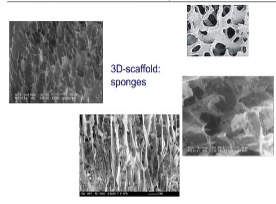
\includegraphics[width=0.5\textwidth]{sponge.jpg}
\caption{\label{fig:sponge}}
\end{figure}
\noindent
Fig \ref{fig:sponge} repair of trabecular bone with 3D-scaffold sponges. 
All of them are artificial scaffolds, while on the top right we have the natural sponge. 
The porosity can be oriented or random, with different geometries.
The scaffold should promote adhesion, proliferation and migration. Hypoxia should be avoided, maybe with early angiogenesis. 
In vivo: in the case of bones, we have osteoblasts adhesion and migration, ECM production. In order to avoid hypoxia and necrotic tissue formation it is required to achieve vascularization, we need to supply oxygen to stimulate angiogenesis. 
In vitro: millimetres not microns, the problem is more tough. We could culture in a bioreactor e.g. chamber with medium forced to go through, or include into the scaffold oxygen donors.

\subsection{Experimental data discussion}
\begin{figure}[h]
\centering
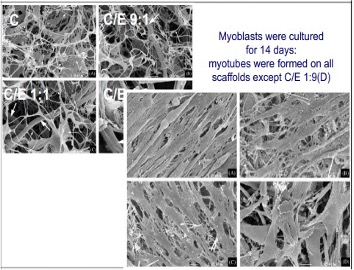
\includegraphics[width=0.5\textwidth]{myoblast.jpg}
\caption{\label{fig:myoblast}}
\end{figure}
\noindent
Fig \ref{fig:myoblast}: muscle regeneration. Use collagen, elastin and glycosaminoglycans. GAGs control water content and mechanical properties. Elastin is required for muscle elasticity, collagen for the strength.
It is necessary to find the optimal ratio among the components.
By changing the ratio,  we have 4 different architectures:
\begin{enumerate}
\item C: sponge, similar to natural behaviour of collagen
\item C/E 9:1: the big fiber starts to appear (elastin)
\item C/E 1:1: similar content
\item C/E 1:9: a lot of big fibers pink fiber: elastin fiber
\end{enumerate}
\noindent
C might not be optimal, as well as C/E 1:9, as they are quite different from biological setting.
In vitro test: after two weeks myoblasts were cultured for 14 days and myotubes were formed on all scaffolds except C/E 1:9(D).  We witness a different organisation of the myotubes; in the last example, myoblasts are not able to organise as the condition is very far from physiology.
By considering the test, the best samples seem to be C/E 9:1 and C/E 1:1 .
\\
\\
\noindent
Tissue engineering is 3D assembly over time of vital tissues-organs by a process involving cells, signals, and the extracellular matrix.
\begin{figure}[h]
\centering
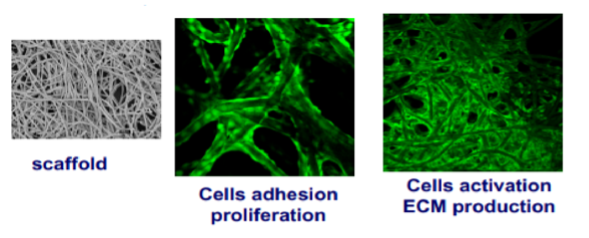
\includegraphics[width=0.6\textwidth]{3D.png}
\caption{\label{fig:3D}}
\end{figure}
In this case we have a scaffold for bone regeneration and osteoblast proliferation (fig \ref{fig:3D}).  The cells (green) are able to adhere, proliferate and migrate. The scaffold is then completely covered in cells. We then witness tissue-specific ECM production, mineralzation. This is a great starting point, but we have to better understand the degradation process of the scaffold and also vascularisation!
How can we check in vivo vascularisation? We need to perform co-culture of osteoblasts (angiogenesis factors + collagenic structure for capillary network formation) and endothelial cells (use empty spaces to assemble as a tube). To obtain a physiological situation we need a careful design.

\section{Scaffold examples}
\subsection{Example 1}
\begin{figure}[h]
\centering
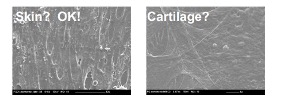
\includegraphics[width=0.6\textwidth]{sk_car.jpg}
\caption{\label{fig:sk_car}}
\end{figure}
Fig \ref{fig:sk_car}: film with same polymers, same architecture, different cells: keratinocytes and chondrocytes. The two films were completely spread.
Cells grown in a flat dish tend to behave as individual cells or forming a monolayer, whereas cells cultured in a 3D space are more likely to assume the characteristics of a particular tissue. 
Cartilage, once grown flat, is almost impossible to shape into joints. The scaffold here, in the case of cartilage, is inducing the loss of the original phenotype,  so it is not biocompatible.
In the case of the skin, it is promising for biocompatibility, very compact and well connected monolayers.

\subsection{Example 2}
\begin{figure}[h]
\centering
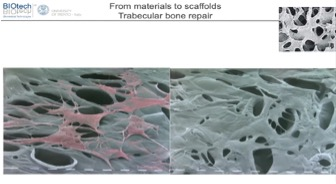
\includegraphics[width=0.5\textwidth]{bone.jpg}
\caption{\label{fig:bone}}
\end{figure}
Fig \ref{fig:bone}: in this case we do not have biocompatibility at all. The cells adhere to the polymer but do not migrate, so we should increase the porosity. 
After few days: we have a multi-layer as result, no migration and no biocompatibility. 

\subsection{Example 3}
\begin{figure}[h]
\centering
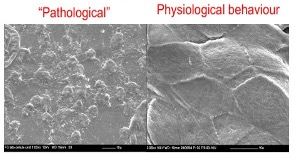
\includegraphics[width=0.5\textwidth]{suine.jpg}
\caption{\label{fig:suine}}
\end{figure}
Fig \ref{fig:suine} suine primary urothelial cells, 6 days after seeding. 
The right image has the geometrical shape of the cells, the phenotype is ok. 
Left: cells don’t connect and are disorganised, so they do not communicate. 
They are more round shaped, so the adherence is not good, there is no activation.




